\documentclass[12pt]{article}
\usepackage{main}
\usepackage{times}
\usepackage{url}
\usepackage{graphicx}
\usepackage{latexsym}
\usepackage{booktabs}
\usepackage{natbib} % Required to change bibliography style to APA
\usepackage{pifont}
\usepackage{enumitem}
\newcommand{\cmark}{\ding{51}}%
\newcommand{\xmark}{\ding{55}}%

\title{Scaling up Stochastic Gradient Descent using Data Parallelism:\\
Application to Horse Racing Prediction using Machine Learning}

\author{
  Ramya Rao Basava \\
  Department of Computer Science \\
  University of British Columbia 
  \\\And
  Ganesh Jawahar \\
  Department of Computer Science \\
  University of British Columbia 
}

\date{}

\begin{document}

\maketitle

\section{Introduction}
In this project, the winner of the Hong Kong Horse Racing is predicted using Machine Learning (ML). In addition to the standard horse and race features, the most frequent words from the match summary for each race are also used as input features. Least squares regression with L2 regularization is used. Given that this is a parallel computing project, apart from trying to get a good accuracy for the ML problem, one of the main aims of the project was to reduce the computation time by parallelizing the Stochastic Gradient Descent (SGD) step. For this, three different approaches were compared as listed below: 

\begin{itemize}[noitemsep, nosep]
 \item Synchronous SGD
 \item Elastic Averaging based Asynchronous SGD
 \item HOGWILD based Asynchronous SGD (based on distributed memory, not shared memory)
\end{itemize}

The overview of the communication structure for the different methods, data processing, the hyperparameters used for different algorithms, MPI parallel environment calls and the results obtained are detailed in the following sections.

\section{Parallelization Algorithms - Communication Structure}
\label{sec:palgs}
\subsection{Synchronous SGD (SYNSGD)}
%\begin{figure}[p]
%\centering
{\centering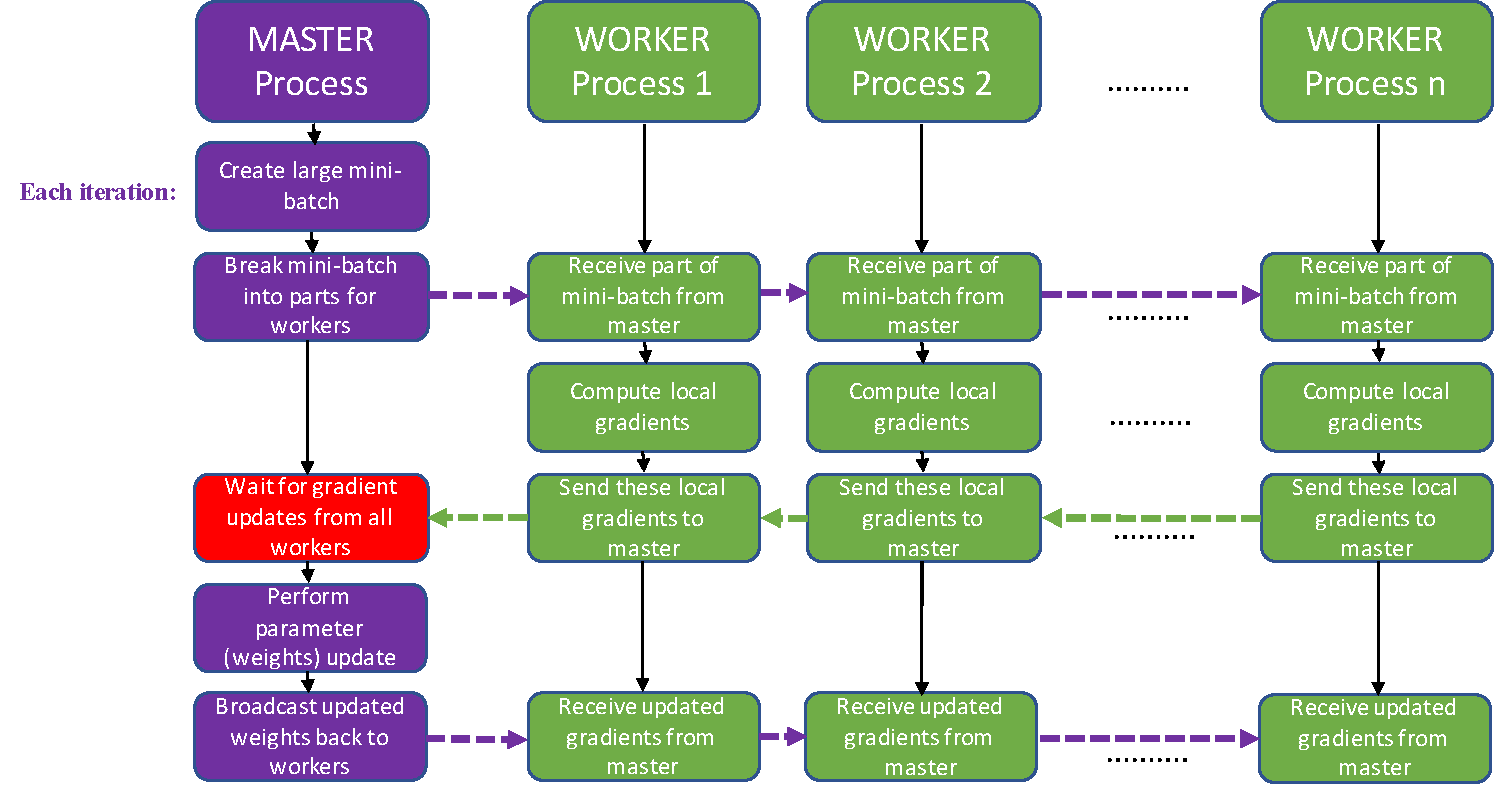
\includegraphics[width=14cm, height=6cm]{images/syncsgd_cstruct.pdf}} \\
%\caption{Communication Structure of Synchronous SGD algorithm. Blue boxes correspond to the actions taken by master while green boxes correspond to the actions taken by worker. Red box corresponds to the action that entail communication bottleneck.}
%\label{fig:archi_syncsgd}
%\end{figure}
In synchronous SGD, for each iteration, the master splits the minibatch equally among workers, waits for workers to return the gradients and then sums all the gradients before performing an update over the master weights. The algorithm executes for several iterations until convergence. %As seen from Figure~\ref{fig:archi_syncsgd}, 
Synchronous SGD entails communication bottleneck at end of each iteration when the master waits for all the workers to complete their task. Thus, \textit{the algorithm is inefficient and is as fast as the slowest worker}.

\subsection{Elastic Averaging based Asynchronous SGD (EASGD)}
%\begin{figure*}[b]
%\centering
{\centering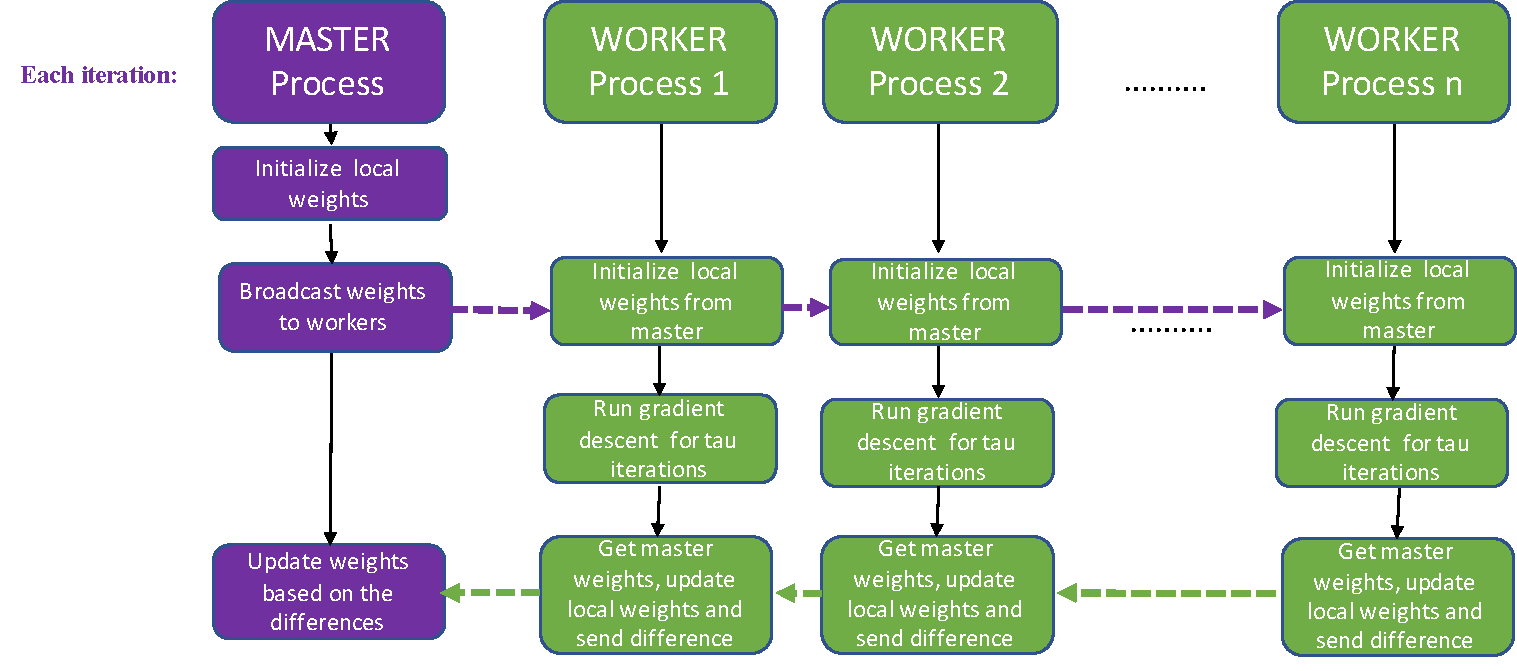
\includegraphics[width=14cm, height=5.5cm]{images/asyncea_cstruct.pdf}} \\
%\caption{Communication Structure of Elastic Averaging based ASynchronous SGD algorithm~\cite{EA2015}.}
%\label{fig:archi_asyncea}
%\end{figure*}
Elastic Averaging based Asynchronous SGD algorithm~\cite{EA2015} lets each worker have a local model and perform SGD on the full dataset. To mitigate the discrepancy between the master and the worker weight, the algorithm defines a elastic force between worker and master weight. This force is more for a worker if its weight is far from master weights and negligible for a worker if its weight is close to master weight. In the latter case, the algorithm lets worker to explore the neighborhood of master's weight space. %This communication pattern is displayed in Figure~\ref{fig:archi_asyncea}.

\subsection{HOGWILD based Asynchronous SGD (HWSGD)}
%\begin{figure*}[b]
%\centering
{\centering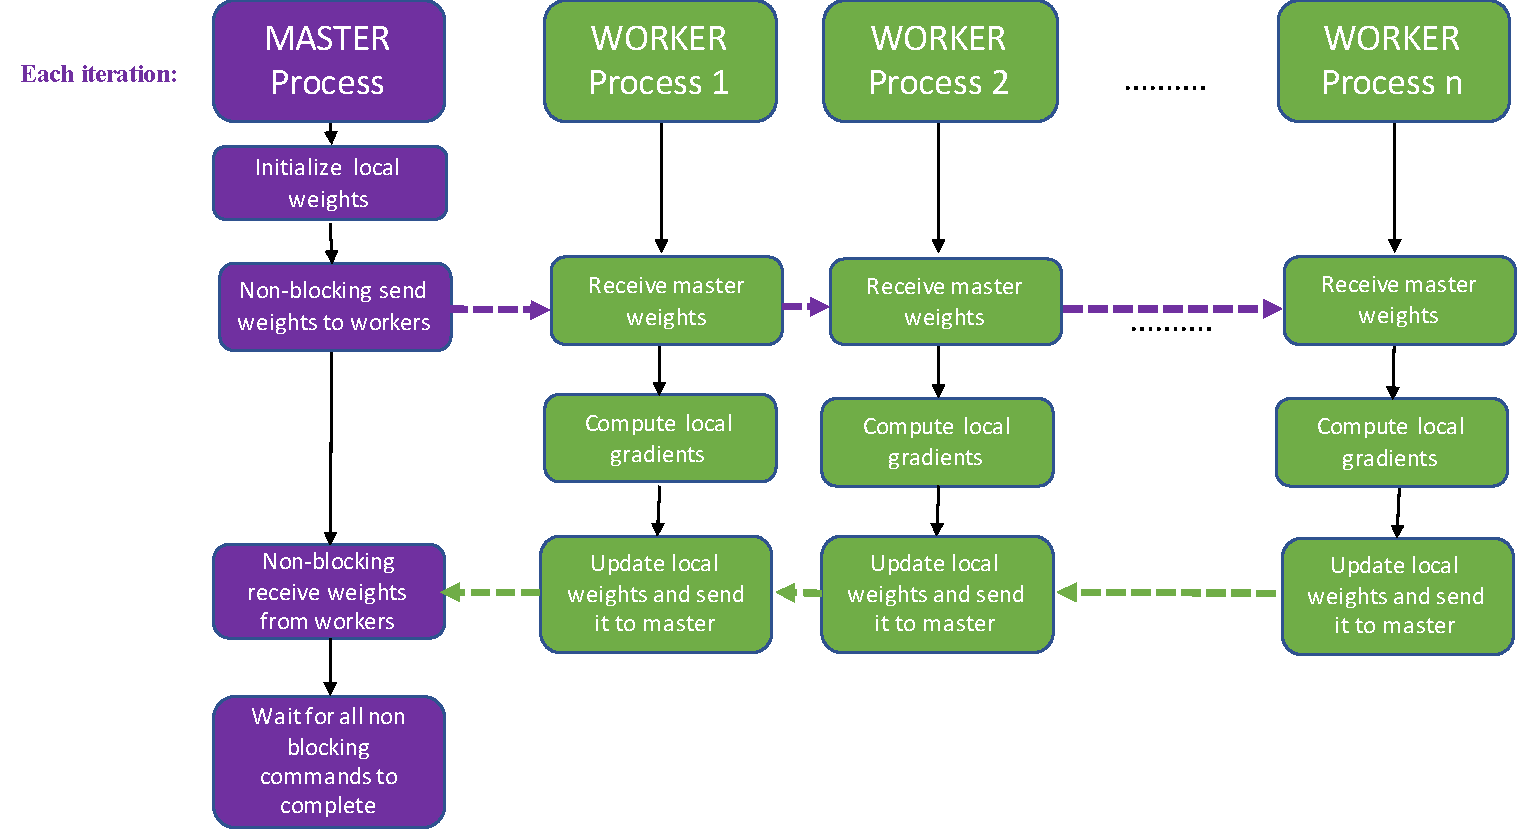
\includegraphics[width=14cm, height=6cm]{images/asynchw_cstruct.pdf}} \\
%\caption{Communication Structure of HOGWILD based ASynchronous SGD algorithm~\cite{Hogwild2011}.}
%\label{fig:archi_asynchw}
%\end{figure*}
In HOGWILD based Asynchronous SGD algorithm~\cite{Hogwild2011}, the master uses non-blocking calls to send weights to worker and receive weights from worker. Such a communication structure lets a worker to overwrite each others progress. The major advantage of this algorithm is that it keeps the workers always busy with work as the master updates its weight lazily with the weight returned by the worker. %The communication pattern of this algorithm is displayed in Figure.~\ref{fig:archi_asynchw}.
 
\section{Horse Racing Prediction - Settings}
\label{sec:settings}
Given a race with a set of horses, the task is to identify the horse from the set that is most likely going to win the race. We use the dataset from Kaggle website.~\footnote{\url{https://www.kaggle.com/alberthkcheng/hong-kong-horse-racing-explained-with-data
}} The statistics of this dataset is displayed below:

\begin{table}[ht]
%\scriptsize
\centering
 \begin{tabular}{llll} 
 \toprule
\textbf{Dataset} & \textbf{No. of Examples} & \textbf{No. of Races} & \textbf{Average horse per race} \\ \midrule
Training & 20514 & 1658 & 12.4 \\
Validation & 2927 & 236 & 12.4 \\
Testing & 5923 & 473 & 12.5 \\
\bottomrule
\end{tabular}
\end{table}

We utilize three categories of features~\footnote{We standardize all the features by removing the mean and scaling to unit variance using Python based scikit-learn library.} (1500/5000 features) for each example:
\begin{itemize}
  \item \textbf{Horse} - Weight, Draw, Horse number, Jockey, Trainer, Actual Weight (includes weight of jockey and gears) (6 features)
  \item \textbf{Race} - Distance, Race course, Race name, Track name, Track condition, Race class and Race number (7 features)
  \item \textbf{Match Summary} - Words that are most frequent in the match summary (1487/4987 features)
\end{itemize}

For performing the machine learning task, we use least squares based \textit{linear regression model with L2 regularization}. We use `Early stopping' to terminate the training when the validation performance is no longer improving after certain number of iterations. The hyperparameters used are given in the table below:
\begin{table}[ht]
%\scriptsize
\centering
 \begin{tabular}{lp{4.0in}l} 
 \toprule
\textbf{Hyperparameter} & \textbf{Description} & \textbf{Value} \\ \midrule
Batch size & Size of the minibatch of training examples for each worker & 200 \\
Maximum Iterations & Maximum number of training iterations before calling off the training & 10000 \\
Lambda & Parameter that controls L2 regularization & 0.5\\
Initial Learning Rate & Learning rate for the weight update step in the stochastic gradient descent algorithm & 0.01 \\
Patience & Parameter for Early Stopping that defines the number of iterations (of poor validation performance) to tolerate before calling off the training & 100 \\
Elasticity Parameter & Parameter for EASGD algorithm that defines the strength of the elastic force between master and worker weight & 0.8 \\
Communication Period & Number of iterations a worker has to wait before synchronization with master for EASGD algorithm & 5 \\
Waitall Period & Number of iterations a master has to wait before calling Waitall() to wait for all nonblocking requests to complete for HWSGD algorithm & 10 \\
\bottomrule
\end{tabular}
\end{table}


\section{MPI Parallel Environment - Settings}
We implement the parallelization algorithms in MPI using C. We use the following MPI commands:
\begin{table}[ht]
\scriptsize
\centering
\begin{tabular}{ccccccc} 
\toprule
\textbf{Command} & \textbf{SYNSGD} (Master) & \textbf{SYNSGD} (Worker) & \textbf{EASGD} (Master) & \textbf{EASGD} (Worker) & \textbf{HWSGD} (Master) & \textbf{HWSGD} (Worker) \\ \midrule
MPI\_Bcast & \cmark & \cmark & \cmark & \cmark & \cmark & \cmark \\
MPI\_Scatterv & \cmark & \cmark & \xmark & \xmark & \xmark & \xmark \\
MPI\_Reduce  & \cmark & \cmark & \cmark & \cmark & \xmark & \xmark \\
MPI\_Isend & \xmark & \xmark & \xmark & \xmark & \cmark & \xmark \\
MPI\_Irecv & \xmark & \xmark & \xmark & \xmark & \cmark & \xmark \\
MPI\_Waitall & \xmark & \xmark & \xmark & \xmark & \cmark & \xmark \\
MPI\_Send & \xmark & \xmark & \xmark & \xmark & \xmark & \cmark \\
MPI\_Recv & \xmark & \xmark & \xmark & \xmark & \xmark & \cmark \\
\bottomrule
\end{tabular}
\end{table}

\section{Results}
\subsection{Comparison of all parallel algorithms}
For the three parallel algorithms given in Section~\ref{sec:palgs}, the computation is run with different number of processors $n=$ 4, 8, 16 and 32. The training terminates once the validation performance reaches an accuracy of 10\%. The training time (in minutes) is recorded for each case and is plotted below for different methods:\\

{\centering
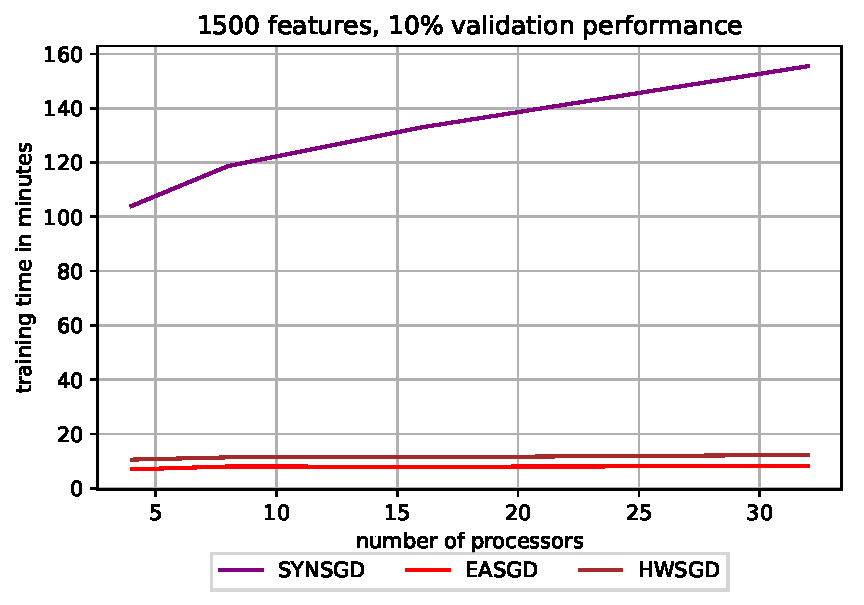
\includegraphics[width=9cm]{images/1500f_10v_def.pdf}\\
}

From the plot, we observe that asynchronous algorithms (EASGD, HWSGD) are faster than synchronous algorithm (SYNSGD) by a large margin. This is mainly due to the communication bottleneck prevalent in SYNSGD when the master waits for all the workers to return the gradients at each iteration. We also find that the training time of SYNSGD increases with number of processors and requires more iterations to converge.

\subsection{Validation and testing results}
The following are the validation and testing results obtained, with the hyper-parameters given in Section~\ref{sec:settings}. The values in the table give the percentage of races predicted correctly in validation and test phases, for the case when $n=16$. 
\begin{table}[ht]
%\scriptsize
\centering
 \begin{tabular}{llll} 
 \toprule
\textbf{Algorithm} & SYNSGD & EASGD & HWSGD \\ \midrule
\textbf{\% Correct in Validation phase} & 10.17 & 11.44 & 10.59 \\
\textbf{\% Correct in Testing phase} & 14.16 & 9.51 & 9.09 \\
\bottomrule
\end{tabular}
\end{table}

\subsection{Comparison of different communication periods for EASGD}
For EASGD, we experiment with different communication periods for different number of processors $n=$ 4, 8, 16 and 32 and stop the training once the validation performance reaches an accuracy of 10\%. The  training  time (in  minutes)  is  recorded  for  each  case. The plot below shows the effect on training time, as the communication period and $n$ are varied:\\

{\centering
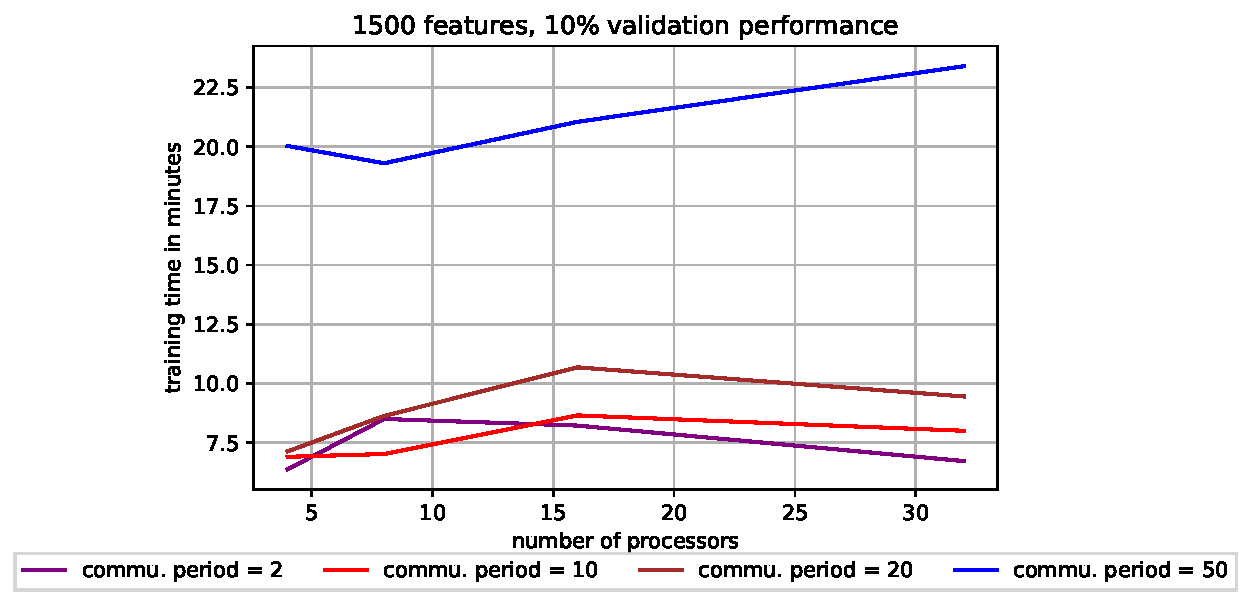
\includegraphics[width=14cm]{images/1500f_10v_ea.pdf}\\
}

From the plot we observe that, when the communication period is high (say 50), the training time increases significantly. This result indicates the possibility that the worker weight becomes stale, when the communication period is high and henceforth, the worker needs more iterations to converge.

\subsection{Comparison of different waitall periods for HWSGD}
For HWSGD, we experiment with different waitall periods for different number of processors $n=$ 4, 8, 16 and 32 and stop the training once the validation performance reaches an accuracy of 10\%. The  training  time (in  minutes)  is  recorded  for  each  case. The plot below shows the effect on training time, as the communication period and $n$ are varied:\\

{\centering
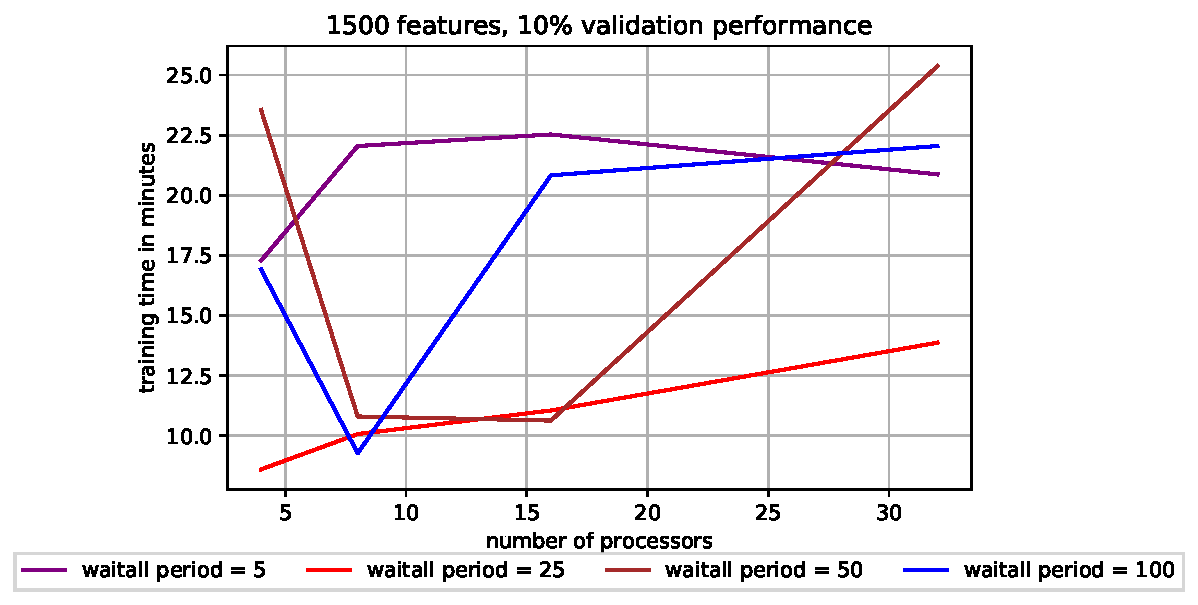
\includegraphics[width=14cm]{images/1500f_10v_hw.pdf}\\
}

From the plot, we observe that the sweet spot of waitall period is 25. For low waitall periods, the training time increases with the increase in number of processors. This indicates that staleness of worker weight increases with increase in number of processors, especially for low waitall periods.


\subsection{Increasing the number of features}
We increase the number of features from 1500 to 5000. EASGD is robust as it outperforms other algorithms by a large margin. 

\begin{table}[ht]
%\scriptsize
\centering
 \begin{tabular}{llll} 
 \toprule
\textbf{Algorithm} & SYNSGD & EASGD & HWSGD \\ \midrule
\textbf{Training time in hours when n = 16} & 11.43 & 1.42 & 6.1 \\
\bottomrule
\end{tabular}
\end{table}


\section{Conclusion}
As it can be seen from the results the test accuracy obtained for SYNSGD is about 14\% and that for EASGD and HWSGD is about 10\%. This is low, which indicates that horse racing prediction is not an easy problem to solve. More in-depth analysis needs to be done to see which features are essentially the best ones to use for this problem. For the parallel computing part, it can be seen that asynchronous methods perform better than the synchronous method, which is expected. Also, EASGD outperforms the other two methods and takes the least amount of compute time, although a small amount of accuracy is lost compared to SYNSGD. Hence, \textit{we recommend Elastic Averaging based Asynchronous SGD (EASGD) as the training algorithm for this ML problem.}


\bibliographystyle{unsrt}
\bibliography{referencefile}

\end{document}
